\RequirePackage[T1]{fontenc}
\documentclass[conference,10pt,letterpaper]{IEEEtran}
\usepackage{amsmath,amssymb,graphicx,booktabs,cite}
\usepackage{tikz}
\usepackage[ruled,vlined,linesnumbered]{algorithm2e}
\SetKwInOut{Input}{Input}
\SetKwInOut{Output}{Output}
\SetKwProg{Stage}{}{}{}
\DontPrintSemicolon
\SetAlgoNlRelativeSize{-1}
\SetInd{0.4em}{0.75em}
\usetikzlibrary{arrows.meta,positioning}
\usepackage{pgfplots}
\usepgfplotslibrary{groupplots}
\pgfplotsset{compat=1.18}
\usepackage[hidelinks]{hyperref}
\hypersetup{pdfauthor={},pdftitle={Exposing Inter-Sample and Intra-Search Parallelism in Layer-Aware Lookahead Construction for 3D FPGA Routing}}
\makeatletter
\newcommand{\tableinput}[1]{\@@input #1 }
\makeatother
\newtheorem{proposition}{Proposition}
\newcommand{\LstmPipeBuild}{$3.207\pm0.147\times$}
\newcommand{\LstmPipeProc}{$1.094\pm0.010\times$}
\newcommand{\LstmFlatBuild}{$3.208\pm0.165\times$}
\newcommand{\LstmFlatProc}{$1.092\pm0.007\times$}
\newcommand{\LstmAltCpuBuild}{$3.167\pm0.071\times$}
\newcommand{\LstmAltCpuProc}{$1.088\pm0.000122\times$}
\newcommand{\LstmStockBuild}{$21.182\pm1.342\times$}
\newcommand{\LstmStockProc}{$1.839\pm0.049\times$}
\newcommand{\StageProcBound}{1.005435}

\newcommand{\GemmNewPipeProc}{$1.102\pm0.004\times$}
\newcommand{\GemmNewStockProc}{$1.921\pm0.003\times$}
\newcommand{\GemmNewPipeBuild}{$3.643\pm0.091\times$}
\newcommand{\GemmNewStockBuild}{$23.524\pm0.120\times$}
\newcommand{\BnnNewPipeProc}{$1.098\pm0.009\times$}
\newcommand{\BnnNewStockProc}{$1.957\pm0.018\times$}
\newcommand{\BnnNewPipeBuild}{$3.197\pm0.116\times$}
\newcommand{\BnnNewStockBuild}{$20.619\pm0.248\times$}

\newcommand{\EstimateGemmShare}{$13.70\%$}
\newcommand{\EstimateGemmZero}{$1.159\times$}
\newcommand{\EstimateGemmReplaced}{$1.110\times$}
\newcommand{\EstimateGemmMeasured}{$1.102\times$}
\newcommand{\EstimateBnnShare}{$14.39\%$}
\newcommand{\EstimateBnnZero}{$1.168\times$}
\newcommand{\EstimateBnnReplaced}{$1.110\times$}
\newcommand{\EstimateBnnMeasured}{$1.098\times$}
\newcommand{\BatchCpuGain}{$1.034\times$}
\newcommand{\BatchCudaGain}{$9.009\times$}

\title{Exposing Inter-Sample and Intra-Search Parallelism in Layer-Aware Lookahead Construction for 3D FPGA Routing}
\author{\IEEEauthorblockN{Anonymous Authors}}
\begin{document}\maketitle
\begin{abstract}Layer-aware lookahead construction for 3D FPGA routing preserves source-relative delay and congestion costs, but its execution order can restrict parallelism both across samples and within a search. We expose these two granularities through context-preserving sample decoupling and whole-pair FP32 bucket waves. Private sample state and original-order reduction provide conditional native wire-map equivalence for STRICT CPU execution. ALT CPU/CUDA use a distinct wave selection rule, qualified separately through complete outputs and native routing. Matched scheduling controls identify cross-group parallelism, while coarser ALT buckets reduce warm BNN batch time by \BatchCudaGain\ on GPU and \BatchCpuGain\ on eight CPU cores. On matched GEMM and BNN runs, ALT CUDA achieves native construction (E2) speedups of \GemmNewPipeBuild\ and \BnnNewPipeBuild\ over eight-core Pipeline. Complete-process speedups are \GemmNewPipeProc\ and \BnnNewPipeProc, respectively. A separate five-arm LSTM cohort gives $3.207\times$ E2 and $1.094\times$ Process speedups over Pipeline. Small-input slowdowns, representative-cost differences and cache applicability delimit these benefits.
\end{abstract}
\begin{IEEEkeywords}3D FPGA, routing lookahead, parallel algorithms, CPU/GPU, source-relative costs\end{IEEEkeywords}
\section{Introduction}
Three-dimensional and multi-die FPGAs expand the design space of programmable interconnects, while placing new demands on the CAD tools used to evaluate them. Recent frameworks support architecture generation, 3D placement and multi-die routing~\cite{lazagna,flatland,multidie}. Lookahead tables summarize delay/congestion costs by resource and destination context. Construction matters when architecture or cost changes invalidate an existing table. Compatible precomputed tables should be reused; our focus is the construction work that remains when such reuse is unavailable.

However, parallel routing does not automatically make lookahead construction parallel. In our locked VPR flow, a prior eight-core GEMM experiment spends 149.56 seconds constructing lookahead---approximately 45\% of its fixed-input process time. Two execution bottlenecks restrict concurrency: barriers between groups containing only a few samples, and fine-grained priority ordering within each search. Simply merging searches or relaxing their ordering is not a drop-in solution. Source/layer-relative recording context and associated delay/congestion representatives must survive reordering. The challenge is to separate removable scheduling constraints from output-defining dependencies.

MultiQueue-based routing parallelizes connection searches through carefully controlled priority relaxation~\cite{multiqueue}; it does not directly provide the sample-recording and reduction semantics of lookahead construction. Multi-die-aware lookahead improves how heuristic costs represent die crossings~\cite{multidie}, addressing the heuristic itself rather than the execution organization studied here. Parallel shortest-path methods already exploit buckets and frontier expansion to balance useful work against scheduling overhead~\cite{delta,gpu_sssp}. Lookahead additionally requires source-relative cells, coupled labels, same-bucket completion and native integration. Caching and sparse sampling can avoid or reduce construction~\cite{vproptions}; we parallelize the retained searches.

Preserving sample identity lets STRICT schedule private searches across groups and reduce in native order. ALT exposes parallelism within each search through whole-pair FP32 waves. On matched GEMM and BNN runs, ALT CUDA speeds native lookahead construction (E2) by $3.643\times$ and $3.197\times$ over optimized eight-core Pipeline, yielding additional complete-process speedups of $1.102\times$ and $1.098\times$, respectively. Against Stock, the full implementation achieves Process speedups of $1.921\times$ and $1.957\times$ on the same runs. An independent historical LSTM comparison gives $3.207\times$ E2 and $1.094\times$ Process speedups over Pipeline. Our contributions are (C1) source-context-preserving cross-group decoupling with explicit reduction conditions, (C2) whole-pair FP32 wave execution with explicit closure and numeric limits, and (C3) native CPU/GPU integration with mechanism controls, route quality validation and measured applicability limits.

\section{Problem and Parallelism Boundary}
\subsection{Layer-Aware Construction}
Let $G=(V,E)$ be the directed routing-resource graph (RRG), with $N=|V|$ nodes and $M=|E|$ edges. Nodes carry resource type, layer, geometry and an indexed delay/congestion cost $w(v)=(d_v,q_v)$. The graph contains planar and cross-layer channels as well as logic, memory and DSP connectivity~\cite{third_dimension,multidie}. PathFinder-style negotiation resolves contention~\cite{pathfinder}; VPR consumes lookahead costs during routing~\cite{vtr8,vtr9}. We accelerate construction of the sampled wire table~\cite{diversity}, not negotiated routing itself.

A group $g=(\ell_s,\sigma,\tau)$ fixes source layer, segment type and channel type. Its ordered samples are source RR nodes $s_{g,j}$ with their native recording contexts. Flattening the native group/sample enumeration gives $J$ jobs indexed by $a$. A job retains its group $g(a)$, ordinal and source $s_a$. Each search can reach all target layers; the target layer is not a separate search. Its recording function $\phi_a(v)$ maps an eligible IPIN to the source-relative cell $u=(\ell_t,\Delta x,\Delta y)$, or to $\bot$ when native geometric filtering excludes it. For a grid of width $X$, height $Y$ and $L$ layers, the dense result domain contains $C=LXY$ cells per sample.

The per-sample result $R_a[u]$ is an occupied pair $(d,q)$ or a missing entry. Delay and congestion are associated representatives produced together by a search; they are not two independently optimized coordinates. Native strict-delay insertion $\oplus$ replaces a missing cell, or replaces an occupied pair only when the incoming delay is smaller. Thus, for each group,
\begin{equation}
 A_g[u]=\mathop{\bigoplus}_{a:g(a)=g}^{\text{native order}}R_a[u],\qquad
 F=\mathcal I\bigl(\mathcal C(\{A_g\})\bigr).
\end{equation}
Here $\mathcal C$ denotes the ordered native group writes and $\mathcal I$ their prescribed interpolation schedule, including missing-cell scan order. This notation represents the actual interleaving of writes and fills, not permission to commute them. The resulting table is indexed by $(\ell_s,\ell_t,\tau,\sigma,\Delta x,\Delta y)$. Source/OPIN preprocessing and derived minima remain in the native outer computation.

\subsection{Necessary Dependencies and Removable Barriers}
Source identity, eligibility, associated pairs and order-sensitive ties define the output. For starts at $x=0$ and $x=5$ reaching an IPIN at $x=6$ with delays 1 and 2, the contributions occupy displacement cells 6 and 1. A multi-source search retaining only the cheaper label at that IPIN loses the second contribution. Separately, inserting $(1,3)$ then $(1,9)$ must retain $(1,3)$ under native strict-delay reduction. Selecting delay and congestion independently could invent a pair no path produced.

In contrast, a search reads the shared graph/costs and its own source context, not another sample's mutable labels. Requiring all searches in group $g$ to finish before exposing group $g+1$ is therefore an execution barrier. Fine-grained priority extraction within a search is another constraint, but changing it also changes representative selection; it requires a separate semantic contract.

\subsection{Relation to Prior Parallelism}
MultiQueue routing controls priority relaxation in connection searches~\cite{multiqueue}; multi-die lookahead improves heuristic treatment of die crossings~\cite{multidie}. Neither directly supplies the sample-recording and ordered reduction boundary above. Delta-stepping and GPU SSSP establish bucket/frontier execution as a way to trade ordering overhead for parallel work~\cite{delta,gpu_sssp}. Atomic minimum supplies the parallel reduction in our GPU implementation. Our specialization retains source-relative cells, coupled cost representatives, closure and native consumption. oneTBB supplies execution primitives~\cite{tbb}; C1 concerns which dependencies those primitives may safely remove. Compatible caches and sparse-sampling \texttt{compressed\_map}~\cite{vproptions} address avoided work; our methods execute the retained samples. Section~\ref{sec:applicability} states their applicability boundaries.

\section{Two Levels of Dependency Decoupling}
\begin{figure}[t]\centering
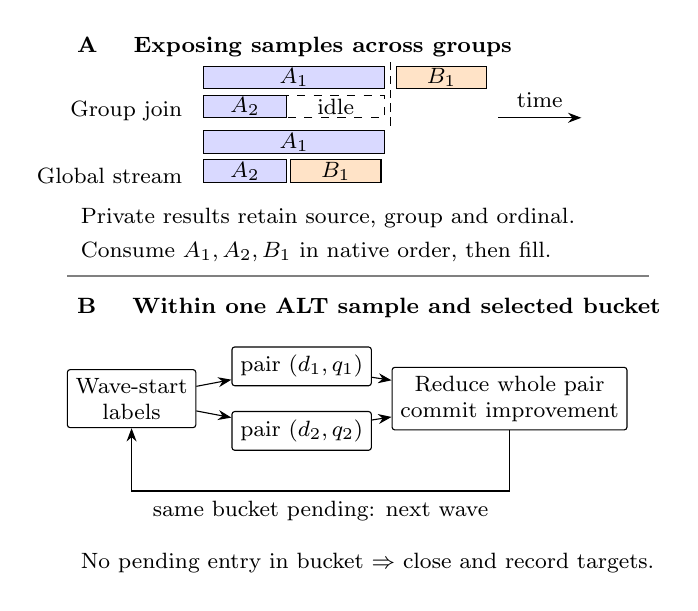
\begin{tikzpicture}[x=0.96cm,y=0.82cm,>=Stealth,font=\footnotesize,
  tile/.style={draw,rounded corners=1pt,inner sep=3pt,align=center}]
\node[anchor=west,font=\bfseries\footnotesize] at (0,0) {A \quad Exposing samples across groups};
\node[anchor=east] at (1.65,-1) {Group join};
\node[anchor=east] at (1.65,-2) {Global stream};
\foreach \y in {-1,-2}{
  \draw[fill=blue!15] (1.8,\y+.35) rectangle (4.2,\y+.70) node[midway] {$A_1$};
  \draw[fill=blue!15] (1.8,\y-.10) rectangle (2.9,\y+.25) node[midway] {$A_2$};
}
\draw[dashed] (2.9,-1.10) rectangle (4.2,-.75) node[midway] {idle};
\draw[densely dashed] (4.28,-1.22)--(4.28,-.20);
\draw[fill=orange!22] (4.35,-.65) rectangle (5.55,-.30) node[midway] {$B_1$};
\draw[fill=orange!22] (2.95,-2.10) rectangle (4.15,-1.75) node[midway] {$B_1$};
\draw[->] (5.7,-1.1)--(6.8,-1.1) node[midway,above] {time};
\node[anchor=west] at (.05,-2.65) {Private results retain source, group and ordinal.};
\node[anchor=west] at (.05,-3.18) {Consume $A_1,A_2,B_1$ in native order, then fill.};
\draw[gray] (0,-3.55)--(7.7,-3.55);
\node[anchor=west,font=\bfseries\footnotesize] at (0,-4.05) {B \quad Within one ALT sample and selected bucket};
\node[tile] (start) at (.85,-5.45) {Wave-start\\labels};
\node[tile] (p1) at (3.1,-4.95) {pair $(d_1,q_1)$};
\node[tile] (p2) at (3.1,-5.95) {pair $(d_2,q_2)$};
\node[tile] (commit) at (5.85,-5.45) {Reduce whole pair\\commit improvement};
\draw[->](start)--(p1);\draw[->](start)--(p2);
\draw[->](p1)--(commit);\draw[->](p2)--(commit);
\draw[->] (commit.south) -- (5.85,-6.88) -- node[below]{same bucket pending: next wave} (.85,-6.88) -- (start.south);
\node[anchor=west] at (.05,-8.0) {No pending entry in bucket $\Rightarrow$ close and record targets.};
\end{tikzpicture}
\caption{Execution dependencies. (A) Illustrative two-worker schedules for groups $A,B$. An idle worker may start $B_1$ while $A_1$ runs. (B) ALT candidates for a destination share a wave snapshot. Committed improvements can reopen the same bucket. Each sample uses one selected search engine.}\label{fig:contracts}
\end{figure}

\subsection{C1: Private Samples and Ordered Consumption}
Algorithm~\ref{alg:c1} overlaps ordered issue, parallel search and ordered merge (Fig.~\ref{fig:contracts}). A token carries index $a$, which identifies the group, ordinal, source and cell map even when a later group starts early. Worker $p$ resets its private queue, visited costs and expanded bits in $S_p$. Its flood reads the shared graph and preserves native geometry, edge eligibility and arithmetic.

\begin{algorithm}[t]
\caption{Bounded STRICT sample pipeline (C1)}\label{alg:c1}
\Input{Graph $G$, ordered starts $(s_{g,j})$, cell maps $\phi_a$, parallelism $P$}
\Output{Sampled wire table $F$}
$\mathcal J\gets\langle(g,j,s_{g,j},\phi_a)\rangle_{(g,j)\text{ in native order}}$\;
$K\gets\min(|\mathcal J|,\max(1,2P)),\quad A_g[\cdot]\gets\bot\quad(\forall g)$\;
\Stage{\textsc{Issue}$()$}{
  \Return $\operatorname{NextIndex}(\mathcal J)$\;
}
\Stage{\textsc{Search}$(a)$}{
  $S_p\gets\operatorname{Reset}(S_p)$\;
  $R_a\gets\operatorname{NativeFlood}(G,s_a,\phi_a,S_p)$\;
  \Return $(a,R_a)$\;
}
\Stage{\textsc{Merge}$(a,R_a)$}{
  $A_{g(a)}[u]\gets A_{g(a)}[u]\oplus R_a[u]\quad(\forall u)$\;
}
$\operatorname{Pipeline}_K(\textsc{Issue},\textsc{Search},\textsc{Merge})$\;
\Return $\mathcal I(\mathcal C(\{A_g\}))$\;
\end{algorithm}

At most $K$ tokens are live. A result $(a,R_a)$ retains its token until the consumer applies $\oplus$ in issue order and releases it. After the join, native group writes and fills follow Section~II. Flat retains all $J$ results for its ordered reduction; Group joins after each group.

\begin{proposition}
If sample selection/context, within-flood visitation and arithmetic are unchanged, occupied recorded delays are finite, and native occupancy, commit and interpolation rules are preserved, private STRICT sample execution followed by original-order strict-delay reduction yields the native wire table.
\end{proposition}
\noindent\emph{Proof.} Each private flood produces the same per-cell representative as its native execution. For an occupied cell, ordered reduction selects the least delay and retains its earliest sample on equal delay:
\begin{equation}
 a^*(g,u)=\arg\min_{a:g(a)=g,\ R_a[u]\ne\bot}(R_a[u].d,a).
\end{equation}
The implementation uses the native missing-state predicate and insertion, not a generic tuple sort. Occupancy and associated congestion therefore agree cell by cell. Identical group writes and interpolation preserve this agreement. Completion order never enters the reduction. $\square$

Changing heap ties, exceptional-value handling or recording geometry violates the premises. The proposition is about wire maps, not route trajectories. ALT below changes the sample engine and does not inherit this proof.

\subsection{C1 Work, Width and Storage}
Let $t_a$ include sample reset, traversal and recording, and $W_g=\sum_{a:g(a)=g}t_a$. Ignoring launch, merge and interference, ideal search schedules obey
\begin{align}
 T_{\rm group}&\geq\sum_g\max\{W_g/P,\max_{a:g(a)=g}t_a\},\\
 T_{\rm global}&\geq\max\{\textstyle\sum_a t_a/P,\max_a t_a\}.
\end{align}
These are lower bounds, not speedup guarantees: an early slow sample can delay ordered consumption and occupy tokens. If $S(N)$ is native private workspace size including its queue, storage beyond the shared graph is $O(P S(N)+KC+|\mathcal G|C+J)$ for Pipeline; Flat replaces $KC$ by $JC$. This exposes the resource tradeoff of retaining independent results. Dense sample-to-group reduction performs $O(JC)$ cell visits; enumeration, group writes and interpolation add their own work. We do not assume a universal $O(M\log N)$ flood cost: actual queue traffic, termination and reset work depend on the native engine and graph.

\subsection{C2: Whole-Pair FP32 Waves}
ALT\_BUCKET\_FP32\_V1 makes the inner ordering rule explicit. A node label $L[v]=(d,q)$ is compared lexicographically:
\begin{equation}
 a\prec b\ \Longleftrightarrow\ a_d<b_d\ \lor\ (a_d=b_d\land a_q<b_q).
\end{equation}
Both coordinates come from one predecessor label plus the destination cost. Native insertion compares delay alone. ALT initializes the source to $(0,0)$, other labels to an infinity sentinel and output cells to missing.

The scheduling key is $B(d)=\mathrm{bits}_{32}(d)\gg h$. Native timings use $h=20$; $h=0$ is a diagnostic exact-delay-key control. Coarsening this key changes which labels are processed together, without quantizing their stored FP32 delays. Costs and generated candidates must be positive normal FP32 or positive zero: negative values, negative zero, subnormals, NaNs and infinities are rejected as numeric inputs/results. Infinity is only internal unreached state. CPU uses round-to-nearest with contraction/fast-math disabled; CUDA explicitly uses round-to-nearest addition. The admission pass checks inter-cluster non-SINK node costs and expansion checks each accumulated pair.

In Algorithm~\ref{alg:c2}, $T_a$ contains the distinct mapped target cells. $\operatorname{Pop}$ removes bucket $b$ from directory $\mathcal D$; only entries whose current key $\pi[u]=b$ are active. $\operatorname{Publish}$ schedules a new key and suppresses duplicate current notifications. CPU filters stale directory entries; CUDA replaces the pending key directly.

\begin{algorithm}[t]
\caption{Whole-pair FP32 waves (C2)}\label{alg:c2}
\Input{$G$, source $s_a$, cell map $\phi_a$, targets $T_a$, key $B$}
\Output{Sample map $R_a$}
$R_a[\cdot]\gets\bot,\quad L[\cdot]\gets(+\infty,+\infty)$\;
\lIf{$T_a=\varnothing$}{\Return $R_a$}
$\pi[\cdot]\gets\bot,\quad\mathcal D,\mathcal H\gets\varnothing,\quad L[s_a]\gets(0,0)$\;
$\operatorname{Publish}(\mathcal D,\pi,s_a,0)$\;
\While{$\mathcal D\ne\varnothing$}{
  $b\gets\min\operatorname{keys}(\mathcal D),\quad X\gets\operatorname{Pop}(\mathcal D,b)$\;
  $U\gets\{u\in X:\pi[u]=b\},\quad \mathcal H\gets\mathcal H\cup U$\;
  $\pi[U]\gets\bot,\quad L^0\gets L,\quad Q\gets L^0$\;
  \ForEach{$u\in U,\;v\in\Gamma(u)$}{
    $z\gets\operatorname{RN}_{32}(L^0[u]+w(v))$\;
    $Q[v]\gets\min_{\prec}(Q[v],z)$\;
  }
  \ForEach{$v$ with $Q[v]\prec L^0[v]$}{
    $L[v]\gets Q[v]$\;
    $\operatorname{Publish}(\mathcal D,\pi,v,B(L[v].d))$\;
  }
  \If{$b\ne\min\operatorname{keys}(\mathcal D)$}{
    \ForEach{$v\in\mathcal H$ with $c=\phi_a(v)\ne\bot$}{
      $R_a[c]\gets\min_{\prec}^{\bot}(R_a[c],L[v])$\;
    }
    $\mathcal H\gets\varnothing$\;
    \lIf{$\operatorname{dom}(R_a)=T_a$}{\Return $R_a$}
  }
}
\Return $R_a$\;
\end{algorithm}

$\Gamma(u)$ lists eligible neighbors in native order, including the SINK stopping rule. $\operatorname{RN}_{32}$ rounds each coordinate; $\min_{\prec}$ selects a whole pair. All proposals read the committed labels $L^0$ before any improvement is published. The snapshot and $Q\gets L^0$ are logical: CPU initializes each proposal on first touch, while CUDA carries forward proposals equal to the committed labels.

Clearing $\pi[U]$ allows same-bucket improvements to enter the next wave. $\mathcal H$ collects expanded nodes until the bucket closes, taking $\min\varnothing=+\infty$. At closure, $\min_{\prec}^{\bot}$ accepts a first mapped IPIN pair in a missing cell and otherwise keeps the smaller pair. $\operatorname{dom}(R_a)$ contains occupied cells; exhaustion leaves unreachable cells missing. Invalid numerics or exceeded guards abort without partial output. FP32 rounding can collapse distinct delays and change which congestion tie survives.

\subsection{CPU/GPU Mapping and Costs}
ALT CPU receives the full job list through the live native interface. An OpenMP dynamic loop assigns independent samples to private scratch arrays with a sparse ordered map of pending buckets. It does not call the STRICT TBB Pipeline. CUDA allocates all $J$ samples together: grid dimension $y$ identifies the sample, while $x$ and 256-thread blocks identify nodes. Each active node thread loops over its own adjacency. Candidate edges are not each assigned a separate thread.

For admitted nonnegative floats the unsigned key
\begin{equation}
 H(d,q)=(\mathrm{uint64}(\mathrm{bits}_{32}(d))\ll32)
          \mathbin{|}\mathrm{bits}_{32}(q)
\end{equation}
orders complete pairs. CUDA uses a 64-bit atomic minimum on each destination proposal; collisions select one actual candidate pair. Separate expansion, commit/minimum-scan, confirmation and advance kernels provide wave boundaries. The commit scan reduces pending keys within each block before one atomic minimum per block; confirmation records IPIN pairs only at closure. Advance scans output occupancy per sample. A host completion-count copy waits each batch round, followed by device synchronization and full output readback/unpacking. The contexts field configures CPU workers; it does not measure CUDA occupancy.

Let $A_{a,k}$ be active nodes, $E_{a,k}$ actually inspected adjacency entries (including rejected edges), $U_{a,k}$ touched destinations and $D_{a,k}$ directory operations in wave $k$. CPU work includes initialization $O(J(N+C))$, $\sum_{a,k}(|A_{a,k}|+|E_{a,k}|+|U_{a,k}|)$, stale-entry filtering, closed-set recording and ordered-directory costs $O(\sum_{a,k}D_{a,k}\log(1+B_{a,k}))$, where $B_{a,k}$ is the number of live directory buckets. Repeated waves can inspect an edge many times. GPU work additionally includes dense scans over allocated $JN$ slots each batch round and closure output scans; for $W$ rounds a useful accounting is
\begin{equation}
 O\!\left(J(N+C)+WJN+\sum_{a,k}|E_{a,k}|+\sum_a H_a C\right),
\end{equation}
where $H_a$ counts closure occupancy scans. Atomic contention, launches and host waits affect elapsed time beyond this work count. Neither formula assumes a single visit per edge.

For the original CUDA representation, arrays require $25JN+8JC$ bytes for labels/proposals, pending, closed flags, mapping and output, plus $8(N+1)+16N+8M$ for CSR/nodes/edges and cost/job metadata. Admission estimates the complete allocation and requires it to fit within 80\% of free device memory; allocation/API errors remain failures. Native ABI shape checks and finite wave/time guards further bound execution. The full 9,595,752-node GEMM graph and all 40 samples pass the live ABI checks and independent output and route qualification.

The host exports current graph/costs and per-sample geometry, calls exactly one chosen backend, then merges returned samples in original order and completes native writes/interpolation. Graph conversion, allocation, transfer, synchronization and output handoff are charged to native E2. Table~\ref{tab:configs} distinguishes executable choices from the two mechanisms. Stock$\to$Pipeline$\to$ALT CUDA is an implementation comparison; it is not a serial two-solver flow or a complete $2\times2$ causal ablation.

\begin{table}[t]\centering
\caption{Execution choices at the common logical boundary.}\label{tab:configs}
\begin{tabular}{lp{2.35cm}p{3.60cm}}\toprule
Configuration & Across samples & Within sample / guarantee\\\midrule
STRICT CPU & Group, Flat or bounded Pipeline & Native flood; conditional wire-map equality\\
ALT CPU & Global dynamic jobs & FP32 waves; separate numeric/QoR qualification\\
ALT CUDA & Full sample batch & Node threads and atomic pairs; ALT CPU output qualification\\\bottomrule
\end{tabular}\end{table}

\section{Experimental Method and Evidence}
\subsection{Frozen Inputs, Cohorts and Resources}
Construction-only controls use separate RRGs and capped route tails. The historical BNN/s38417 study compared Stock, Flat and both ALT backends. LSTM seed2, used previously for CPU evaluation, is a same-family holdout from ALT tuning. It shares BNN's architecture and has its own netlist, placement and RRG.

The Stock comparisons retain their original seed1 inputs: width100 for GEMM, width120 for BNN. LSTM also uses width120; all three have two layers and 40 samples (Table~\ref{tab:qor}). The Stock and engine comparisons use separate allocations, each with eight physical cores and NUMA0 memory binding on a Xeon Platinum 8462Y+, one H100 80GB, a 10-CPU quota and 200GiB RAM. The earlier native ALT cohorts use eight physical cores in one NUMA node on Gold 6530 and one H100 80GB. Solvers execute sequentially, with rotated arm order and fresh processes. Shared hosts are not exclusive; cohorts are not pooled. The baseline is VTR commit \texttt{0b912334fdd8}, release build, assertion level 2.

\subsection{Timing and Statistical Policy}
E1 is sample service; CUDA ends it before final ABI output copy. E2 is native \texttt{MapLookahead::compute}: conversion, preparation/service, output handoff, group merge, interpolation, source/OPIN and derived minima. Process adds RR XML loading, initialization, routing, checking/STA and uniform serialization. Independent route readback, pre-generated RRG, packing and placement are excluded. Caches are not flushed.

For paired repeat $r$, $s_r=T_{c,r}/T_{a,r}$. We report mean and sample SD of ratios and raw seconds ($n=3$). SD is not a confidence interval; repeats are processes, not designs or seeds. Stock E2 precision is 0.01s; other E2 timers are high resolution. Profiles are outside formal timing.

\subsection{Qualification and Attribution}
STRICT checks wire-map bytes under its proposition. ALT checks complete CPU/CUDA pairs and maps, then each route through independent original-VPR FULL/STA with unchanged route SHA, zero overuse, and CPD/wirelength within $+5\%$ of controls: Flat/Stock for LSTM, Stock/Pipeline for the GEMM/BNN Stock comparisons. All formal ALT measurements disable capture and CPU-reference verification. The separate engine comparison qualifies complete outputs against frozen maps and compares both ALT routes to their own repeat's Pipeline route.

Retained bounding-box notification repairs can change route trajectories despite identical maps; a unique complete cause is not established. Stock ratios describe the implementation combination. Shared-repair Flat/Pipeline/ALT comparisons better isolate construction.

\section{Results and System Interpretation}
\subsection{STRICT Cross-Sample Parallelism}
On the prior eight-core GEMM cohort, STRICT Pipeline reduces construction from 149.56 to 20.95 seconds and achieves $1.638\pm0.005\times$ paired Process speedup over Stock; Group takes 37.88 seconds. Construction is about 45\% of Stock Process. Matched Group/Flat/Pipeline controls isolate C1 from other Stock repairs.

\begin{figure}[t]\centering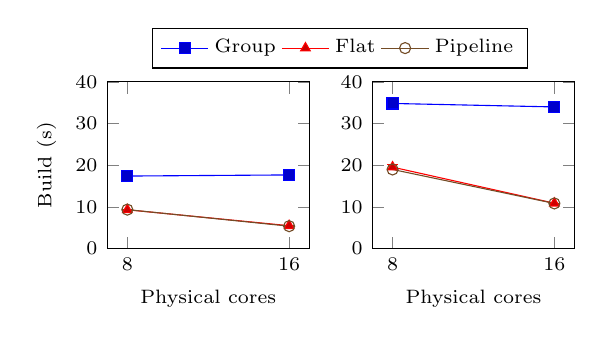
\begin{tikzpicture}
\begin{groupplot}[group style={group size=2 by 1,horizontal sep=0.8cm},width=4.15cm,height=3.7cm,xtick={8,16},xmin=7,xmax=17,ymin=0,ymax=40,xlabel={Physical cores},ylabel={Build (s)},label style={font=\scriptsize},tick label style={font=\scriptsize},legend style={font=\scriptsize,at={(1.15,1.08)},anchor=south,legend columns=3},error bars/y dir=both,error bars/y explicit]
\nextgroupplot[title={},ylabel={Build (s)}]
\addplot+[mark=square*] coordinates {(8,17.413333333333334) +- (0,0.3250128202599597) (16,17.683333333333334) +- (0,0.3257811126098835)};
\addplot+[mark=triangle*] coordinates {(8,9.32) +- (0,0.15394804318340596) (16,5.506666666666667) +- (0,0.030550504633038766)};
\addplot+[mark=o] coordinates {(8,9.363333333333333) +- (0,0.10598742063723142) (16,5.3933333333333335) +- (0,0.08082903768654771)};
\legend{Group,Flat,Pipeline}
\nextgroupplot[title={},ylabel={}]
\addplot+[mark=square*] coordinates {(8,34.82333333333333) +- (0,0.3181718613160717) (16,33.99) +- (0,0.6602272336097627)};
\addplot+[mark=triangle*] coordinates {(8,19.553333333333335) +- (0,0.6217180497084931) (16,10.896666666666667) +- (0,0.040414518843273746)};
\addplot+[mark=o] coordinates {(8,18.993333333333332) +- (0,0.11503622617824955) (16,10.846666666666668) +- (0,0.04041451884327389)};
\end{groupplot}
\end{tikzpicture}

\caption{Construction means and sample SD, three processes per arm/point. Same-cohort Group/Flat/Pipeline controls on BNN (left) and DLA (right); capped routing tails do not establish full-route legality. Error bars are small at this scale.}\label{fig:causal}\end{figure}

With ten groups of four samples, Group limits concurrency to four searches. At eight cores, BNN Group/Flat/Pipeline take $17.41\pm0.33$, $9.32\pm0.15$ and $9.36\pm0.11$ s (Fig.~\ref{fig:causal}). At sixteen cores the times are 17.68/5.51/5.39 s. DLA shows the same pattern (34.82/19.55/18.99 s at eight cores). Both global schedulers benefit from exposing work across groups. Separate eight-core BNN-2D controls take 7.75/4.23/4.16 s on a different graph.

\subsection{Wave Scheduling: Concurrency Versus Work}
\begin{table}[t]\centering\caption{Historical BNN40 bucket comparison. Work profiles and warm complete-batch seconds on eight physical cores and one H100.}\label{tab:waves}
\begin{tabular}{lrr}\toprule Metric & Shift 0 & Shift 20\\\midrule
\tableinput{tables/waves.tex}\midrule\tableinput{tables/batch_seconds.tex}\bottomrule\end{tabular}\end{table}
Table~\ref{tab:waves} links independently profiled work to warm complete-batch service on the same BNN40 input. Coarsening the ALT bucket reduces total waves $9.112\times$ and maximum sample waves $10.627\times$. Eligible edge work rises $0.3504\%$, while edge-weighted frontier grows $6.6484\times$. The eight-core CPU gains \BatchCpuGain\ and the GPU gains \BatchCudaGain. Wider fronts expose more simultaneous work between synchronization points. Both shifts retain FP32 labels and agree on all sample outputs on this batch.

Service includes reset, search, closure and materializing outputs, including GPU readback and synchronization. Load, preparation and verification fall outside the timer. Each time is the median of three process medians, each over three warm batches with profiling and witnesses off. Speedups here divide those medians. Native E2 additionally charges graph conversion and outer lookahead construction.

\subsection{Matched Native Process and Construction}
\begin{table*}[t]\centering\caption{Complete native Process seconds and directly paired speedups, mean $\pm$ sample SD ($n=3$). S: Stock; P: Pipeline; C: ALT CUDA. GEMM/BNN are one new allocation; LSTM is a separate historical cohort.}\label{tab:matchedproc}
\begin{tabular}{lrrrrrr}\toprule Workload & Stock (s) & Pipeline (s) & ALT CUDA (s) & S/P & P/C & S/C\\\midrule
\tableinput{tables/matched_process.tex}\bottomrule\end{tabular}\end{table*}
\begin{table*}[t]\centering\caption{Native lookahead construction E2 seconds and directly paired speedups for the same runs as Table~\ref{tab:matchedproc}; mean $\pm$ sample SD, $n=3$.}\label{tab:matchede2}
\begin{tabular}{lrrrrrr}\toprule Workload & Stock (s) & Pipeline (s) & ALT CUDA (s) & S/P & P/C & S/C\\\midrule
\tableinput{tables/matched_e2.tex}\bottomrule\end{tabular}\end{table*}
ALT CUDA achieves E2 speedups of \GemmNewPipeBuild\ for GEMM and \BnnNewPipeBuild\ for BNN over Pipeline (Tables~\ref{tab:matchedproc}--\ref{tab:matchede2}). E2 accounts for \EstimateGemmShare\ and \EstimateBnnShare\ of mean Pipeline Process time. Holding the mean remainder fixed, eliminating E2 would give \EstimateGemmZero\ and \EstimateBnnZero\ Process speedups. Substituting mean CUDA E2 instead gives \EstimateGemmReplaced\ for each workload. Actual paired Process speedups are \GemmNewPipeProc\ and \BnnNewPipeProc; other stages can also change.


\subsection{Matched Native Engine and Backend Comparison}
\begin{table}[t]\centering
\caption{Independent eight-core/H100 cohort. Directly paired speedups ($n=3$, mean $\pm$ sample SD). P: Pipeline, A: ALT CPU, C: ALT CUDA.}\label{tab:engines}
\begin{tabular}{@{}lrrr@{}}\toprule Case and scope & P/A & A/C & P/C\\\midrule
\tableinput{tables/engine_ratios.tex}\bottomrule\end{tabular}\end{table}
Changing the CPU engine and scheduler together yields Process ratios near one (Table~\ref{tab:engines}), including $0.973\pm0.074$ on GEMM. Holding the ALT rule fixed, CUDA speeds construction by $4.690\times$ on GEMM and $4.331\times$ on BNN. The corresponding Process speedups are $1.146\times$ and $1.162\times$.

\subsection{Native LSTM: Five Matched Configurations}
\begin{table}[t]\centering\caption{Historical LSTM native seconds, mean $\pm$ sample SD ($n=3$); five arms on its own rotated eight-core/H100 cohort.}\label{tab:lstm}
\begin{tabular}{lrr}\toprule Method & E2 & Process\\\midrule
\tableinput{tables/lstm.tex}\bottomrule\end{tabular}\end{table}
On historical LSTM, CUDA achieves \LstmPipeBuild\ E2 and \LstmPipeProc\ Process speedups over Pipeline. Against matched ALT CPU the speedups are \LstmAltCpuBuild\ and \LstmAltCpuProc. Table~\ref{tab:lstm} includes the full five-arm comparison.

\subsection{Semantics, QoR and Size Dependence}
\begin{table}[t]\centering\caption{Native qualification: nodes/edges in millions; CPD/WL changes (\%) against Stock; $\Delta q$ counts final-map congestion-word changes against STRICT. All cases have two layers and 40 samples; LSTM is historical.}\label{tab:qor}
\begin{tabular}{lrrrrr}\toprule Case & $N/10^6$ & $M/10^6$ & CPD & WL & $\Delta q$\\\midrule
\tableinput{tables/qualification_compact.tex}\bottomrule\end{tabular}\end{table}
Complete ALT CPU/CUDA samples and maps agree. Stock/Pipeline maps also agree. ALT changes only congestion representatives (Table~\ref{tab:qor}), with zero delay or missing-state differences. Each route passes independent FULL/STA with zero overuse and preserves its own SHA. All native runs meet their respective CPD/WL gates.

On the historical BNN cohort, CUDA achieves $3.274\pm0.222\times$ E2 and $1.091\pm0.011\times$ Process speedups over Flat. On small s38417 the corresponding ratios fall to $0.274\pm0.032\times$ and $0.912\pm0.016\times$. Initialization, scans and launches can outweigh search savings.

\subsection{Closest Alternative and Cache Applicability}\label{sec:applicability}
The locked \texttt{compressed\_map} requires one layer, excluding these two-layer graphs. Separable remains unmeasured. Ordinary caching supports valid reuse: 36 fixed-input cache hits passed independent FULL/STA. Our timings cover fresh construction.

\section{Scope and Limitations}
STRICT equality remains conditional; ALT route qualification covers tested graphs, not a universal QoR bound. Three process repetitions, shared hosts and same-family architectures limit generalization. Controls and ALT retain RRG no-fanin diagnostics: FULL/STA validates actual routes, not every graph-generation choice. Dense state, scans and launch costs bound GPU applicability. The evidence supports complementary mechanisms, not independent multiplicative C1/C2 effects or an automatic backend selector.

\section{Conclusion}
Preserving source context exposes independent samples for ordered native reduction. Within a search, whole-pair FP32 waves expose parallel work at a separately qualified semantic boundary. CUDA speeds complete Process over Pipeline by \GemmNewPipeProc\ and \BnnNewPipeProc\ in the GEMM/BNN Stock comparisons. In the independent engine comparison, GPU mapping of the same ALT rule gives $1.146\times$ and $1.162\times$ over ALT CPU. The small-input slowdown bounds applicability.

\section*{Content Generated by AI}
OpenAI Codex (GPT-6) assisted manuscript text, figures, artifact scripts and experimental analysis. Authors are responsible for verification and submission.

\clearpage
\bibliographystyle{IEEEtran}
\bibliography{references}
\end{document}
